\RequirePackage{luatex85}
\documentclass[tikz, border=10pt]{standalone}

\usepackage[compat=1.1.0]{tikz-feynman}

\begin{document}

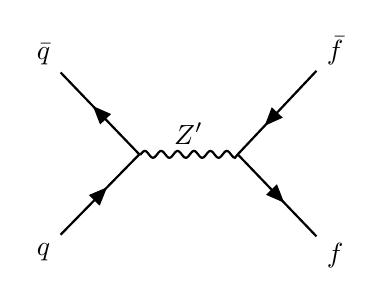
\begin{tikzpicture}[thick]
 \begin{feynman}
  \vertex (origin);
  \vertex [right=1.25cm of origin] (X);
  \vertex [above left=1cm and 1cm of origin] (q1) {\(\bar{q}\)};
  \vertex [below left=1cm and 1cm of origin] (q2) {\(q\)};
  \vertex [above right=1cm and 1cm of X] (f1) {\(\bar{f}\)};
  \vertex [below right=1cm and 1cm of X] (f2) {\(f\)};
  \diagram* {
  (origin) -- [boson, edge label={\(Z^{\prime}\)}] (X) -- [anti fermion] (f1),
  (X) -- [fermion] (f2),
  (origin) -- [fermion] (q1),
  (q2) -- [fermion] (origin),
  };
 \end{feynman}
\end{tikzpicture}
\end{document}
